\documentclass[margin=3pt,
  convert,
  convert={
    outext=.png,
    command=\unexpanded{
      pdftocairo -r 300 -png \infile % 将生成的pdf文件转换为png图像
    }
  }
  ]{standalone}

\usepackage{tkz-euclide}

\begin{document}

% 勾股树
% TODO:应该使用循环进行绘制,但目前还无法实现
%       敬请各位网友能给出修改意见
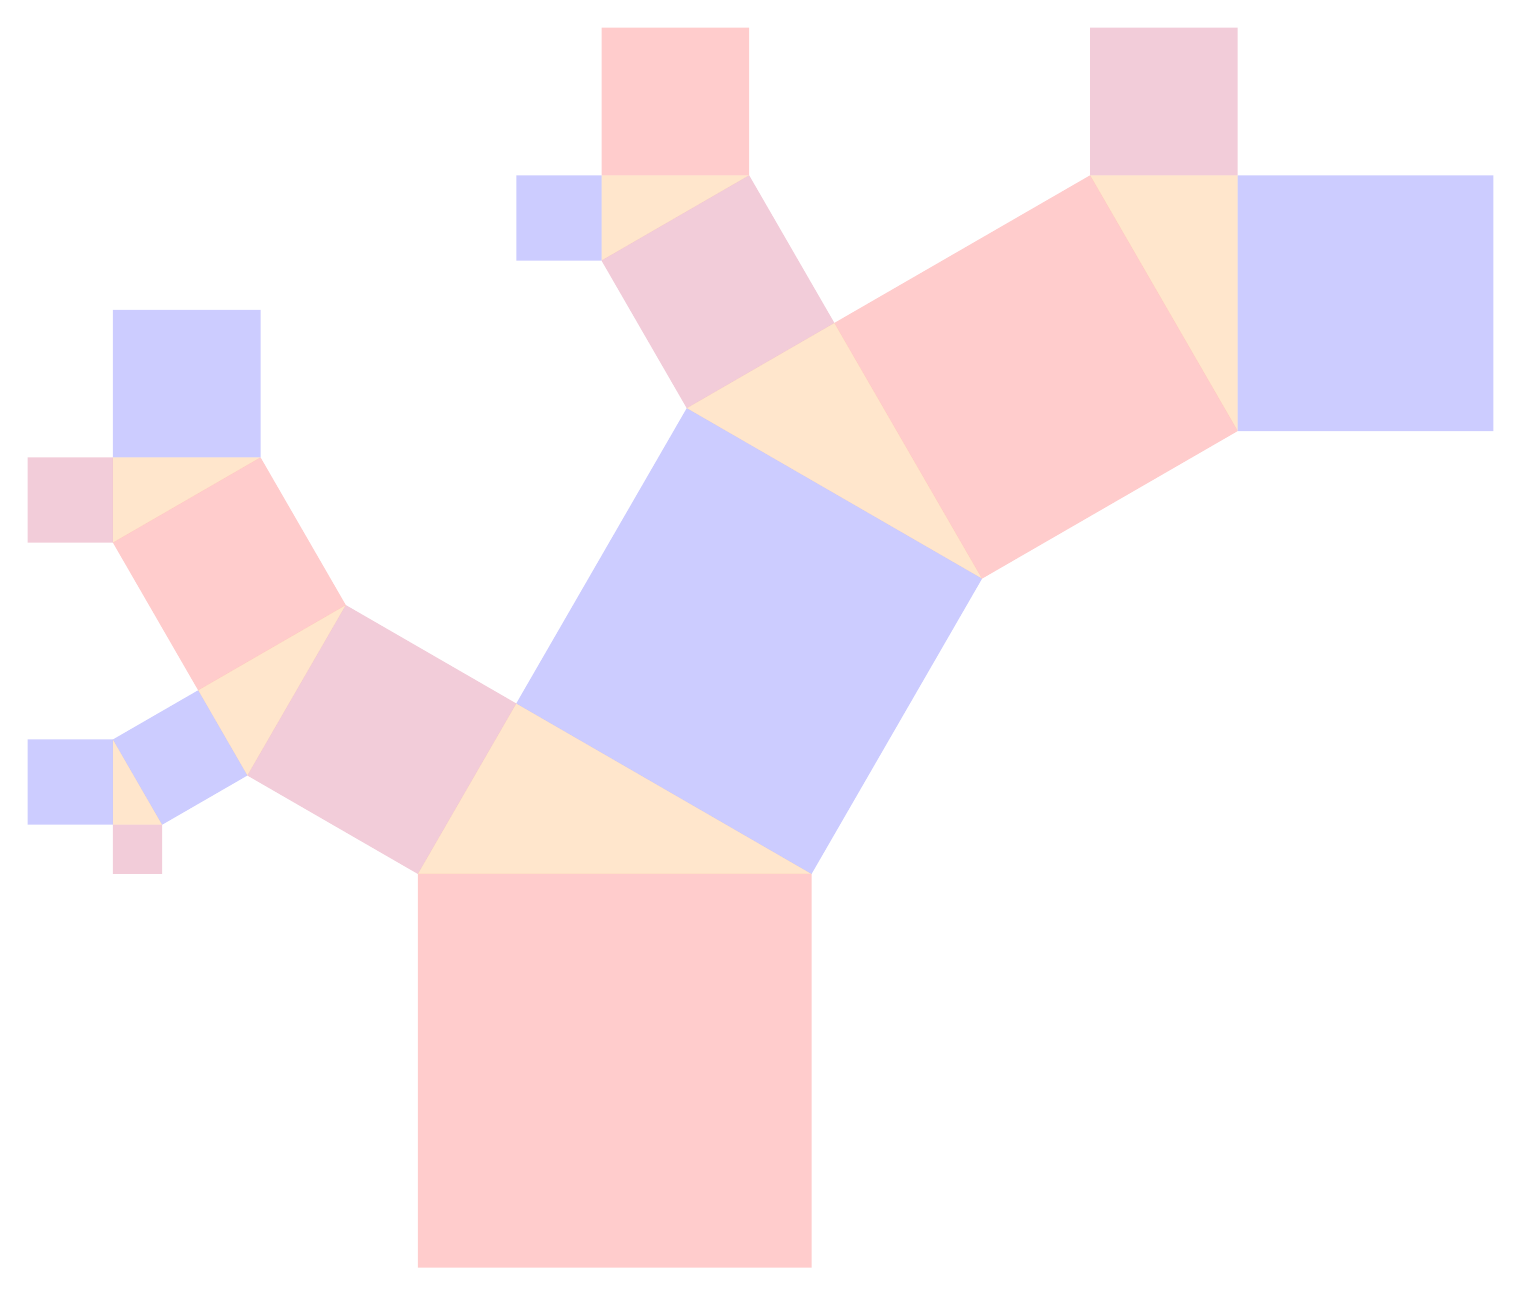
\begin{tikzpicture}  
  % 定义B和A点
  \tkzDefPoint(0,0){B}
  \tkzDefPoint(5,0){A}
  % 计算三角形顶点E
  \tkzDefTriangle[two angles= 60 and 30](B,A) \tkzGetPoint{E}
  % 定义矩形
  \tkzDefSquare(A,B)\tkzGetPoints{C}{D}
  \tkzDefSquare(E,A)\tkzGetPoints{H}{I}
  \tkzDefSquare(B,E)\tkzGetPoints{F}{G}  
  % 绘制填充矩形
  \tkzFillPolygon[fill = red!20 ](A,B,C,D)
  \tkzFillPolygon[fill = blue!20 ](E,A,H,I)
  \tkzFillPolygon[fill = purple!20](B,E,F,G)
  \tkzFillPolygon[fill = orange,opacity=.2](B,A,E)

  % 计算三角形顶点E
  \tkzDefTriangle[two angles= 60 and 30](I,H) \tkzGetPoint{E}
  % 定义矩形
  \tkzDefSquare(E,H)\tkzGetPoints{A}{B}
  \tkzDefSquare(I,E)\tkzGetPoints{C}{D}  
  % 绘制填充矩形
  \tkzFillPolygon[fill = red!20 ](E,H,A,B)
  \tkzFillPolygon[fill = purple!20 ](I,E,C,D)
  \tkzFillPolygon[fill = orange,opacity=.2](I,H,E)

  % 计算三角形顶点E
  \tkzDefTriangle[two angles= 60 and 30](G,F) \tkzGetPoint{E}
  % 定义矩形
  \tkzDefSquare(E,F)\tkzGetPoints{H}{I}
  \tkzDefSquare(G,E)\tkzGetPoints{J}{K}  
  % 绘制填充矩形
  \tkzFillPolygon[fill = red!20 ](E,F,H,I)
  \tkzFillPolygon[fill = blue!20 ](G,E,J,K)
  \tkzFillPolygon[fill = orange,opacity=.2](G,F,E)

  % 计算三角形顶点E
  \tkzDefTriangle[two angles= 60 and 30](B,A) \tkzGetPoint{E}
  % 定义矩形
  \tkzDefSquare(E,A)\tkzGetPoints{F}{G}
  \tkzDefSquare(B,E)\tkzGetPoints{L}{M}  
  % 绘制填充矩形
  \tkzFillPolygon[fill = blue!20 ](E,A,F,G)
  \tkzFillPolygon[fill = purple!20 ](B,E,L,M)
  \tkzFillPolygon[fill = orange,opacity=.2](B,A,E)

  % 计算三角形顶点E
  \tkzDefTriangle[two angles= 60 and 30](D,C) \tkzGetPoint{E}
  % 定义矩形
  \tkzDefSquare(E,C)\tkzGetPoints{A}{B}
  \tkzDefSquare(D,E)\tkzGetPoints{N}{O}  
  % 绘制填充矩形
  \tkzFillPolygon[fill = red!20 ](E,C,A,B)
  \tkzFillPolygon[fill = blue!20 ](D,E,N,O)
  \tkzFillPolygon[fill = orange,opacity=.2](D,C,E)

  % 计算三角形顶点E
  \tkzDefTriangle[two angles= 60 and 30](I,H) \tkzGetPoint{E}
  % 定义矩形
  \tkzDefSquare(E,H)\tkzGetPoints{C}{D}
  \tkzDefSquare(I,E)\tkzGetPoints{P}{Q}  
  % 绘制填充矩形
  \tkzFillPolygon[fill = blue!20 ](E,H,C,D)
  \tkzFillPolygon[fill = purple!20 ](I,E,P,Q)
  \tkzFillPolygon[fill = orange,opacity=.2](I,H,E)

  % 计算三角形顶点E
  \tkzDefTriangle[two angles= 60 and 30](K,J) \tkzGetPoint{E}
  % 定义矩形
  \tkzDefSquare(E,J)\tkzGetPoints{H}{I}
  \tkzDefSquare(K,E)\tkzGetPoints{R}{S}  
  % 绘制填充矩形
  \tkzFillPolygon[fill = blue!20 ](E,J,H,I)
  \tkzFillPolygon[fill = purple!20 ](K,E,R,S)
  \tkzFillPolygon[fill = orange,opacity=.2](K,J,E)
\end{tikzpicture}

\end{document}

%%% Local Variables:
%%% mode: latex
%%% TeX-master: t
%%% End:
